\pdfminorversion=4
\documentclass[10pt]{beamer}\usepackage[]{graphicx}\usepackage[]{color}
%% maxwidth is the original width if it is less than linewidth
%% otherwise use linewidth (to make sure the graphics do not exceed the margin)
\makeatletter
\def\maxwidth{ %
  \ifdim\Gin@nat@width>\linewidth
    \linewidth
  \else
    \Gin@nat@width
  \fi
}
\makeatother

\definecolor{fgcolor}{rgb}{0.345, 0.345, 0.345}
\newcommand{\hlnum}[1]{\textcolor[rgb]{0.686,0.059,0.569}{#1}}%
\newcommand{\hlstr}[1]{\textcolor[rgb]{0.192,0.494,0.8}{#1}}%
\newcommand{\hlcom}[1]{\textcolor[rgb]{0.678,0.584,0.686}{\textit{#1}}}%
\newcommand{\hlopt}[1]{\textcolor[rgb]{0,0,0}{#1}}%
\newcommand{\hlstd}[1]{\textcolor[rgb]{0.345,0.345,0.345}{#1}}%
\newcommand{\hlkwa}[1]{\textcolor[rgb]{0.161,0.373,0.58}{\textbf{#1}}}%
\newcommand{\hlkwb}[1]{\textcolor[rgb]{0.69,0.353,0.396}{#1}}%
\newcommand{\hlkwc}[1]{\textcolor[rgb]{0.333,0.667,0.333}{#1}}%
\newcommand{\hlkwd}[1]{\textcolor[rgb]{0.737,0.353,0.396}{\textbf{#1}}}%

\usepackage{framed}
\makeatletter
\newenvironment{kframe}{%
 \def\at@end@of@kframe{}%
 \ifinner\ifhmode%
  \def\at@end@of@kframe{\end{minipage}}%
  \begin{minipage}{\columnwidth}%
 \fi\fi%
 \def\FrameCommand##1{\hskip\@totalleftmargin \hskip-\fboxsep
 \colorbox{shadecolor}{##1}\hskip-\fboxsep
     % There is no \\@totalrightmargin, so:
     \hskip-\linewidth \hskip-\@totalleftmargin \hskip\columnwidth}%
 \MakeFramed {\advance\hsize-\width
   \@totalleftmargin\z@ \linewidth\hsize
   \@setminipage}}%
 {\par\unskip\endMakeFramed%
 \at@end@of@kframe}
\makeatother

\definecolor{shadecolor}{rgb}{.97, .97, .97}
\definecolor{messagecolor}{rgb}{0, 0, 0}
\definecolor{warningcolor}{rgb}{1, 0, 1}
\definecolor{errorcolor}{rgb}{1, 0, 0}
\newenvironment{knitrout}{}{} % an empty environment to be redefined in TeX

\usepackage{alltt}
%% O comando acima foi necessario porque o PDF nao abria no acrobat do
%% windows, dava o erro 131. Provavelmente devido as figuras em
%% PDF. Agora ele gera um PDF versao 1.4, ao inves da versao 1.5

\usetheme[compress]{PaloAlto}
\usecolortheme{sidebartab} % crane

\usepackage[brazilian]{babel}
\usepackage[T1]{fontenc}
\usepackage[utf8]{inputenc}
\usepackage{graphicx}
\usepackage{hyperref}
\usepackage[scaled]{beramono} % truetype: Bistream Vera Sans Mono
%\usepackage{inconsolata}
\usepackage{amsmath}
\usepackage{xfrac}
\usepackage{tikz}
\usepackage{xcolor}
\usepackage{multirow}
\usepackage{multicol}
\usepackage{tikz}
\usetikzlibrary{arrows, decorations.pathmorphing, backgrounds, fit,
  positioning, calc, trees, plotmarks}

\setbeamertemplate{footline}[frame number] % mostra o numero dos slides
\setbeamertemplate{navigation symbols}{} % retira a barra de navegacao

\usepackage{xspace}
\providecommand{\eg}{\textit{e.g.}\xspace}
\providecommand{\ie}{\textit{i.e.}\xspace}
\providecommand{\R}{\textsf{R}\xspace}
\newcommand{\mb}[1]{\mathbf{#1}}
\newcommand{\bs}[1]{\boldsymbol{#1}}
\providecommand{\E}{\text{E}}
\providecommand{\Var}{\text{Var}}
\providecommand{\DP}{\text{DP}}
\providecommand{\EP}{\text{EP}}
\providecommand{\N}{\text{N}}
\theoremstyle{definition}
\newtheorem*{mydef}{Definição}
\newtheorem*{mythm}{Teorema}

\title{Teste de hipótese para uma população}
\author[]{Fernando de Pol Mayer}
\institute[UFPR]{Laboratório de Estatística e Geoinformação (LEG) \\
  Departamento de Estatística (DEST) \\
  Universidade Federal do Paraná (UFPR)}
\date{}
\logo{\includegraphics[width=1.6cm]{../img/ufpr-logo.png}}
\titlegraphic{\includegraphics[width=1cm]{../img/CC_by-nc-sa_88x31.png}\\
  \tiny
  \href{https://creativecommons.org/licenses/by-nc-sa/4.0/deed.pt_BR}{Este
    conteúdo está disponível por meio da Licença Creative Commons 4.0
    (Atribuição/NãoComercial/PartilhaIgual)}}

\AtBeginSection[]
{
  \begin{frame}
    \frametitle{Plano de aula}
    \tableofcontents[currentsection]
  \end{frame}
}

\AtBeginSubsection[]
{
  \begin{frame}
    \frametitle{Plano de aula}
    \tableofcontents[currentsection,currentsubsection]
  \end{frame}
}
\IfFileExists{upquote.sty}{\usepackage{upquote}}{}
\begin{document}





\begin{frame}
\maketitle
%\titlepage
\end{frame}

\begin{frame}{Sumário}
\tableofcontents
\end{frame}

\section{Introdução}

\begin{frame}{Introdução}
  Na \textbf{inferência estatística} os dois principais objetivos são:
  \\~\\
  \begin{enumerate}
  \item \textbf{Estimar} um parâmetro populacional
  \item \textbf{Testar} uma hipótese ou afirmativa sobre um parâmetro
    populacional
  \end{enumerate}
\end{frame}

\begin{frame}{Introdução}
  \begin{block}{Hipótese}
    É uma afirmativa sobre uma propriedade da população
  \end{block}
  \begin{block}{Teste de hipótese}
    É um procedimento para se testar uma afirmativa sobre uma
    propriedade da população
  \end{block}
  \vspace{1em}
  Permite tomar \textbf{decisões} sobre a população com base em
  informações de dados amostrais.
\end{frame}

\section[Componentes]{Componentes dos testes de hipótese}

\begin{frame}{Tipos de hipóteses}
  \begin{block}{Hipótese nula $H_0$}
    É uma afirmativa de que o valor de um parâmetro populacional é
    \textbf{igual} a algum valor especificado. (O termo \textit{nula} é
    usado para indicar nenhuma mudança, nenhum efeito). Ex.:
    \begin{itemize}
    \item $\mu = 170$ cm
    \item $p = 0,5$
    \end{itemize}
  \end{block}
\begin{block}{Hipótese alternativa $H_a$}
    É uma afirmativa de que o parâmetro tem um valor, que, de alguma
    forma, difere da hipótese nula. Ex.:
    \begin{itemize}
    \item $\mu \neq 170$ \qquad $\mu < 170$ \qquad $\mu > 170$
    \end{itemize}
  \end{block}
\end{frame}

\begin{frame}{Tipos de hipóteses}
  Quando fazemos um teste de hipótese, chegamos a um dos dois
  possíveis resultados: \\~\\
  \begin{itemize}
  \item \textbf{Rejeitar $H_0$}: em favor da hipótese alternativa $H_a$
  \item \textbf{Não rejeitar $H_0$}: e conclui-se que não existem
    diferenças
  \end{itemize}
  % \pause
  \vspace{1em}
  \begin{alertblock}{Atenção!}
    \begin{itemize}
    \item O termo \textbf{aceitar} a hipótese nula é filosoficamente
      incorreto, pois não se pode aceitar uma hipótese baseada apenas em
      evidências amostrais (mesmo em um teste de hipótese formal).
      \item E ainda existe um \textbf{erro} associado a todo teste de
        hipótese \ldots
    \end{itemize}

  \end{alertblock}
\end{frame}

\begin{frame}{Erro do tipo I e do tipo II}
  \textbf{Erro do tipo I}: rejeitar uma hipótese nula verdadeira. A
  probabilidade de cometer esse erro é dada por $\alpha$. \\~\\
  \textbf{Erro do tipo II}: não rejeitar uma hipótese nula falsa. A
  probabilidade de cometer esse erro é dada por $\beta$.
  \begin{table}[H]
    \centering
    \begin{tabular}{c|cc}
      \hline
       & \textbf{$H_o$ verdadeira} & \textbf{$H_o$ falsa} \\
       \hline
       \textbf{Não rejeitar $H_0$} & Decisão correta & Erro tipo II \\
       \textbf{Rejeitar $H_0$} & Erro tipo I & Decisão correta \\
       \hline
    \end{tabular}
  \end{table}
  Portanto, o valor de $\alpha$ determina a chance de erro do teste de
  hipótese.
\end{frame}

\begin{frame}{Nível de significância $\alpha$}
  O nível de significância $\alpha$ é a probabilidade de cometermos um
  erro do tipo I. \\~\\
  Este valor é determinado \textbf{antes} de se iniciar o teste, e
  determina o nível de risco que pode ser tolerado ao se rejeitar uma
  hipótese nula que é verdadeira. \\~\\
  Valores comuns de $\alpha$ são 0,10; 0,05 e 0,01.
\end{frame}

\begin{frame}{Testes unilaterais e bilaterais}
  Uma hipótese do tipo
  \begin{itemize}
  \item[] $H_0 = $
  \item[] $H_a \neq$
  \end{itemize}
  é \textbf{bilateral}
  \begin{figure}[H]
    \centering
    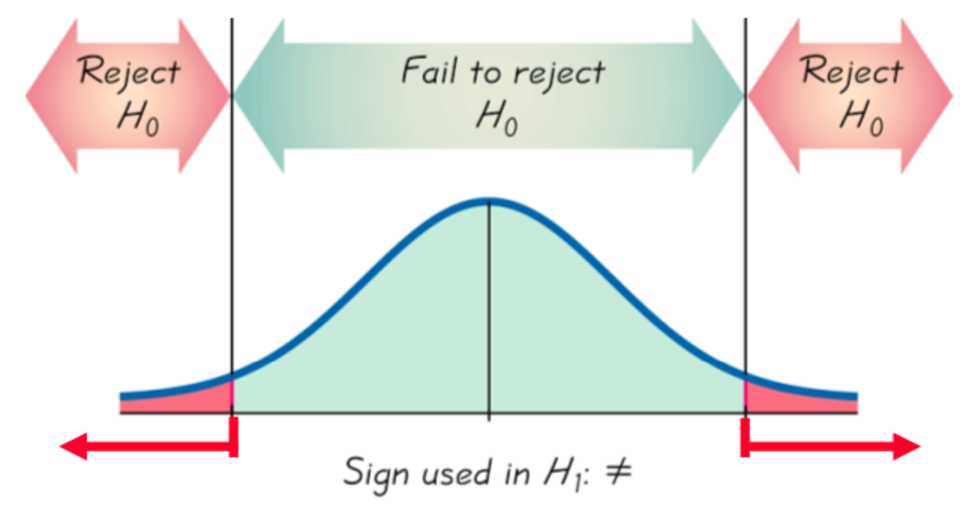
\includegraphics[width=.8\textwidth]{bilateral2}
  \end{figure}
\end{frame}

\begin{frame}{Testes unilaterais e bilaterais}
  Uma hipótese do tipo
  \begin{itemize}
  \item[] $H_0 \geq $
  \item[] $H_a <$
  \end{itemize}
  é \textbf{unilateral à esquerda}
  \begin{figure}[H]
    \centering
    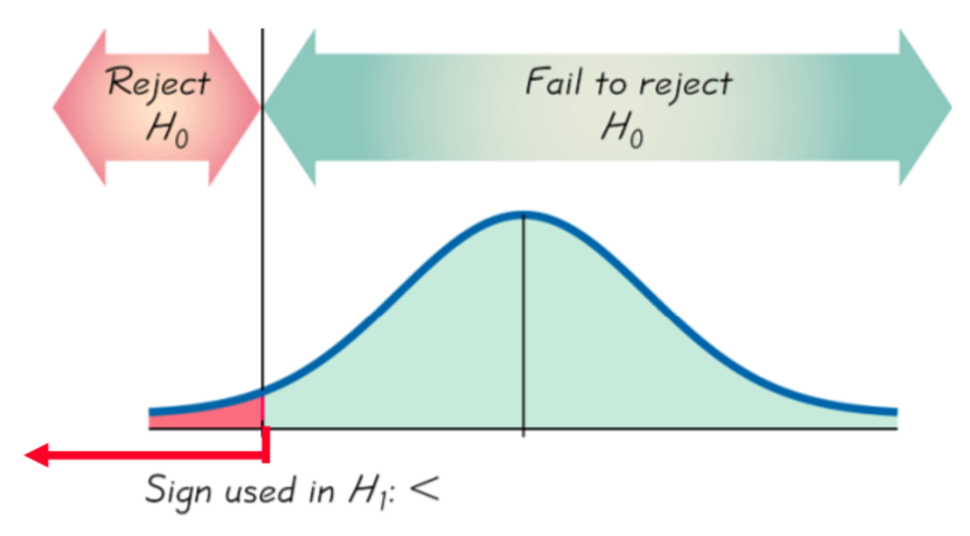
\includegraphics[width=.8\textwidth]{uni_esq2}
  \end{figure}
\end{frame}

\begin{frame}{Testes unilaterais e bilaterais}
  Uma hipótese do tipo
  \begin{itemize}
  \item[] $H_0 \leq $
  \item[] $H_a >$
  \end{itemize}
  é \textbf{unilateral à direita}
  \begin{figure}[H]
    \centering
    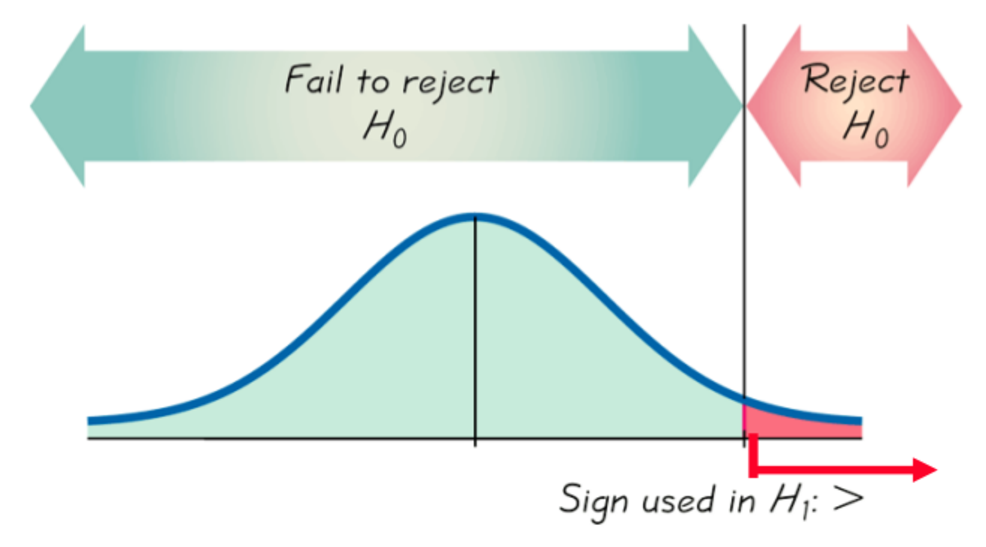
\includegraphics[width=.8\textwidth]{uni_dir2}
  \end{figure}
\end{frame}

\begin{frame}{Testes unilaterais e bilaterais}
  A \textbf{região crítica} de um teste de hipótese é a área de
  \textbf{rejeição} da hipótese nula\\~\\
  O \textbf{valor crítico} é o valor que divide a área de rejeição da
  área de não rejeição de $H_0$. Depende:
  \begin{itemize}
  \item da distribuição amostral da estimativa testada
  \item do valor de $\alpha$
  \end{itemize}
\end{frame}

\begin{frame}{Estatística de teste}
  A \textbf{estatística de teste} é um valor usado para tomar a decisão
  sobre a hipótese nula.\\~\\
  É encontrada pela conversão da estatística amostral em um escore ($z$
  ou $t$), com a suposição de que a hipótese nula seja verdadeira.\\~\\
  Se:
  \begin{itemize}
  \item A estatística de teste cair \textbf{dentro} da região crítica
    $\rightarrow$ \textbf{rejeita $H_0$}
  \item A estatística de teste cair \textbf{fora} da região crítica
    $\rightarrow$ \textbf{não rejeita $H_0$}
  \end{itemize}
\end{frame}

\begin{frame}{Estatística de teste}
  Exemplo: estatística de teste para uma média com $\sigma$ conhecido
  \begin{equation*}
    z_{calc} = \frac{\bar{x} - \mu_0}{\sigma/\sqrt{n}}
  \end{equation*}
  Este valor \textbf{calculado} deve ser comparado com um \textbf{valor
    crítico} de $z_{crit}$, obtido a partir da tabela da distribuição
  $\text{N}(0,1)$.\\~\\
  Se:
  \begin{itemize}
  \item $|z_{calc}| > |z_{crit}|$ $\rightarrow$ \textbf{rejeita $H_0$}
  \item $|z_{calc}| < |z_{crit}|$ $\rightarrow$ \textbf{não rejeita $H_0$}
  \end{itemize}
\end{frame}

\begin{frame}{Procedimentos gerais para um teste de hipótese}
\begin{enumerate}
\item Definir a hipótese nula ($H_0$) e a alternativa ($H_a$)
\item Definir um nível de \textbf{significância} $\alpha$ (ex.: $\alpha
  = 0,05$), que irá determinar o nível de \textbf{confiança}
  $100(1-\alpha)\%$ do teste
\item Determinar a \textbf{região de rejeição} com base no nível de
  significância $\rightarrow$ valor crítico
\item Calcular a \textbf{estatística de teste}, sob a hipótese nula
  $\Rightarrow$ valor calculado
  % \begin{equation*}
  %   z_{calc} = \frac{\bar{x} - \mu_0}{\sigma/\sqrt{n}}
  % \end{equation*}
\item Rejeitar a hipótese nula se a estatística de teste calculada
  estiver dentro da região de rejeição $\Rightarrow$ |valor calculado| >
  |valor crítico|
\end{enumerate}
\end{frame}

\section{Testes de hipótese para a média $\mu$}

\subsection{$\sigma$ conhecido}

\begin{frame}{Testes de hipótese para a média: $\sigma$ conhecido}
  Quando temos os seguintes requisitos: \\~\\
  \begin{enumerate}
  \item Temos uma AAS
  \item $\sigma$ é conhecido
  \item A população tem distribuição normal ou $n>30$
  \end{enumerate}
  \vspace{1em}
  podemos usar o Teorema Central do Limite para afirmar que a média
  segue uma distribuição normal, e a \textbf{estatística de teste} é
  dada por
  \begin{equation*}
    z_{calc} = \frac{\bar{x} - \mu_0}{\sigma/\sqrt{n}}
  \end{equation*}
  onde $\mu_0$ é o valor de teste na hipótese nula.
\end{frame}

\begin{frame}{Testes de hipótese para a média: $\sigma$ conhecido}
  \textbf{Procedimentos gerais para um teste de hipótese com $\sigma$
    conhecido}
\begin{enumerate}
\item Definir a hipótese nula ($H_0$) e a alternativa ($H_1$)
\item Definir um nível de \textbf{significância} $\alpha$ (ex.: $\alpha
  = 0,05$), que irá determinar o nível de \textbf{confiança}
  $100(1-\alpha)\%$ do teste
\item Determinar a \textbf{região de rejeição} com base no nível de
  significância $\rightarrow$ $z_{crit}$
\item Calcular a \textbf{estatística de teste}, sob a hipótese nula
  \begin{equation*}
    z_{calc} = \frac{\bar{x} - \mu_0}{\sigma/\sqrt{n}}
  \end{equation*}
\item Rejeitar a hipótese nula se a estatística de teste calculada
  estiver dentro da região de rejeição ($|z_{calc}| > |z_{crit}|$)
\end{enumerate}
\end{frame}

\begin{frame}[fragile]{Testes de hipótese para a média: $\sigma$ conhecido}
  \textbf{Exemplo}: \\~\\
  Uma máquina de encher embalagens de café está funcionando
  adequadamente se colocar 700 g em cada embalagem. \\~\\
  Para verificar a calibração da máquina, uma empresa coletou uma
  amostra de 40 embalagens, que resultou em uma média de 698 g. Sabe-se
  que o desvio-padrão do enchimento da máquina é de 10 g. \\~\\
  Teste a hipótese de o peso médio das embalagens na população ser 700
  g, com um nível de significância de 5\%.
  \pause
\begin{knitrout}\footnotesize
\definecolor{shadecolor}{rgb}{0.969, 0.969, 0.969}\color{fgcolor}\begin{kframe}
\begin{verbatim}
$`valor critico`
[1] -1.96  1.96

$`estatistica de teste`
[1] -1.2649

$decisao
[1] "nao rejeita H0"
\end{verbatim}
\end{kframe}
\end{knitrout}
\end{frame}

% Morettin pg 244
\begin{frame}[fragile]{Testes de hipótese para a média: $\sigma$ conhecido}
  \textbf{Exemplo}: \\~\\
  Um fabricante de lajotas introduz um novo material em sua fabricação e
  acredita que aumentará a resistência média, que é de 206
  kg. \\~\\
  A resistência das lajotas tem distribuição normal com desvio-padrão de
  12 kg. Retirou-se uma amostra de 30 lajotas, e
  obteve-se uma média amostral de 210 kg. \\~\\
  Ao nível de 10\%, o fabricante pode afirmar que a resistência média de
  suas lajotas aumentou?
  \pause
\begin{knitrout}\footnotesize
\definecolor{shadecolor}{rgb}{0.969, 0.969, 0.969}\color{fgcolor}\begin{kframe}
\begin{verbatim}
$`valor critico`
[1] 1.2816

$`estatistica de teste`
[1] 1.8257

$decisao
[1] "rejeita H0"
\end{verbatim}
\end{kframe}
\end{knitrout}
\end{frame}

\subsection[$\sigma$ desconhe.]{$\sigma$ desconhecido}

\begin{frame}{Testes de hipótese para a média: $\sigma$ desconhecido}
  Quando temos os seguintes requisitos: \\~\\
  \begin{enumerate}
  \item Temos uma AAS
  \item $\sigma$ é \textbf{desconhecido}
  \item A população tem distribuição normal ou $n>30$
  \end{enumerate}
  \vspace{1em}
  usamos a distribuição $t$ como \textbf{estatística de teste}, dada por
  \begin{equation*}
    t_{calc} = \frac{\bar{x} - \mu_0}{s/\sqrt{n}}
  \end{equation*}
  com $n-1$ \textbf{graus de liberdade}, e onde $\mu_0$ é o valor de
  teste na hipótese nula.
\end{frame}

\begin{frame}{Testes de hipótese para a média: $\sigma$ desconhecido}
  \textbf{Procedimentos gerais para um teste de hipótese com $\sigma$
    desconhecido}
\begin{enumerate}
\item Definir a hipótese nula ($H_0$) e a alternativa ($H_1$)
\item Definir um nível de \textbf{significância} $\alpha$ (ex.: $\alpha
  = 0,05$), que irá determinar o nível de \textbf{confiança}
  $100(1-\alpha)\%$ do teste
\item Determinar a \textbf{região de rejeição} com base no nível de
  significância $\rightarrow$ $t_{crit}$ (com $gl = n-1$)
\item Calcular a \textbf{estatística de teste}, sob a hipótese nula
  \begin{equation*}
    t_{calc} = \frac{\bar{x} - \mu_0}{s/\sqrt{n}}
  \end{equation*}
\item Rejeitar a hipótese nula se a estatística de teste calculada
  estiver dentro da região de rejeição ($|t_{calc}| > |t_{crit}|$)
\end{enumerate}
\end{frame}

\begin{frame}[fragile]{Testes de hipótese para a média: $\sigma$ desconhecido}
  \textbf{Exemplo}: \\~\\
  A vida média das lâmpadas produzidas por uma empresa era de
  1120 horas. \\~\\
  Uma amostra de 8 lâmpadas extraída recentemente apresentou
  a vida média de 1070 horas, com desvio-padrão de 125 horas, e
  distribuição próxima da normal. \\~\\
  Testar a hipótese de que a vida média
  das lâmpadas não tenha se alterado, ao nível de 1\% de significância.
  \pause
\begin{knitrout}\footnotesize
\definecolor{shadecolor}{rgb}{0.969, 0.969, 0.969}\color{fgcolor}\begin{kframe}
\begin{verbatim}
$`valor critico`
[1] -3.4995  3.4995

$`estatistica de teste`
[1] -1.1314

$decisao
[1] "nao rejeita H0"
\end{verbatim}
\end{kframe}
\end{knitrout}
\end{frame}

\begin{frame}[fragile]{Testes de hipótese para a média: $\sigma$ desconhecido}
  \textbf{Exemplo}: \\~\\
  Querendo determinar a quantidade média de nicotina dos
  cigarros, uma empresa retirou uma amostra de 25 cigarros e obteve os
  seguintes resultados:
  \begin{equation*}
    \bar{x} = 38 \, \text{mg} \qquad s^2 = 0,25 \, \text{mg}^2
  \end{equation*}
  Ao nível de 5\%, teste se a quantidade média de nicotina pode ser
  considerada inferior a 40 mg.
  \pause
\begin{knitrout}\footnotesize
\definecolor{shadecolor}{rgb}{0.969, 0.969, 0.969}\color{fgcolor}\begin{kframe}
\begin{verbatim}
$`valor critico`
[1] -1.7109

$`estatistica de teste`
[1] -20

$decisao
[1] "rejeita H0"
\end{verbatim}
\end{kframe}
\end{knitrout}
\end{frame}

\begin{frame}[fragile]{Testes de hipótese para a média: $\sigma$ desconhecido}
  \textbf{Exemplo}: \\~\\
  Uma máquina é projetada para fazer esferas de aço de 1 cm de raio. Uma
  amostra de 10 esferas é produzida, e tem raio médio de 1,004
  cm, com $s = 0,003$. \\~\\
  Há razões para suspeitar que a máquina esteja produzindo esferas com
  raio maior que 1 cm? (Use um nível de significância de 10\%).
  \pause
\begin{knitrout}\footnotesize
\definecolor{shadecolor}{rgb}{0.969, 0.969, 0.969}\color{fgcolor}\begin{kframe}
\begin{verbatim}
$`valor critico`
[1] 1.383

$`estatistica de teste`
[1] 4.2164

$decisao
[1] "rejeita H0"
\end{verbatim}
\end{kframe}
\end{knitrout}
\end{frame}

\section{Testes de hipótese para a proporção $p$}

\begin{frame}{Testes de hipótese para a proporção $\pi$}
  A proporção amostral
  \begin{equation*}
    p = \frac{x}{n} = \frac{\text{número de sucessos}}{\text{total de
        tentativas}}
  \end{equation*}
  é a \textbf{melhor estimativa} para a proporção populacional $\pi$
  \\~\\
  Já vimos que quando ambas condições são satisfeitas
  \begin{itemize}
  \item $np \geq 5$
  \item $n(1-p) \geq 5$
  \end{itemize}
  a distribuição binomial das proporções amostrais pode ser
  \textbf{aproximada} por uma distribuição normal com com média $\mu =
  np$ e desvio-padrão $\sigma = \sqrt{np(1-p)}$
\end{frame}

\begin{frame}{Testes de hipótese para a proporção $\pi$}
  Quando temos os seguintes requisitos:
  \begin{enumerate}
  \item Temos uma AAS
  \item As condições para a distribuição binomial são satisfeitas
    \begin{itemize}
    \item as tentativas são independentes
    \item há duas categorias de resultado (``sucesso'', ``fracasso'')
    \item a probabilidade de sucesso $p$ permanece constante
    \end{itemize}
  \item $n\pi_0 \geq 5$ e $n(1-\pi_0) \geq 5$
  \end{enumerate}
  podemos usar a distribuição normal como aproximação da binomial, e
  portanto, usamos a \textbf{estatística de teste}
  \begin{equation*}
    z_{calc} = \frac{p - \pi_0}{\sqrt{\frac{\pi_0(1-\pi_0)}{n}}}
  \end{equation*}
  onde $\pi_0$ é o valor de proporção de teste na hiótese nula.
\end{frame}

\begin{frame}{Testes de hipótese para a proporção $\pi$}
  \textbf{Procedimentos gerais para a construção de um teste de hipótese
    para a proporção $\pi$} \\~\\
  \begin{enumerate}
  \item Definir a hipótese nula ($H_0$) e a alternativa ($H_1$)
  \item Determine o valor de $p = \frac{x}{n}$
  \item Verifique se $n\pi_0 \geq 5$ e $n(1-\pi_0) \geq 5$
  \item Definir um nível de \textbf{significância} $\alpha$ (ex.: $\alpha
    = 0,05$), que irá determinar o nível de \textbf{confiança}
    $100(1-\alpha)\%$ do teste
  \item Determinar a \textbf{região de rejeição} com base no nível de
    significância $\rightarrow$ $z_{crit}$
  \item Calcular a \textbf{estatística de teste}, sob a hipótese nula
    \begin{equation*}
      z_{calc} = \frac{p - \pi_0}{\sqrt{\frac{\pi_0(1-\pi_0)}{n}}}
    \end{equation*}
  \item Rejeitar a hipótese nula se a estatística de teste calculada
    estiver dentro da região de rejeição ($|z_{calc}| > |z_{crit}|$)
  \end{enumerate}
\end{frame}

\begin{frame}{Testes de hipótese para a proporção $\pi$}
  % triola pg 334
  Exemplo: Uma empresa desenvolveu um método de seleção de gênero, e
  afirma que, com a utilização deste método, a proporção de nascer uma
  menina é maior do que 50\%. Para pais que utilizaram o método, dos 726
  bebês nascidos, 668 eram meninas.\\~\\
  Use este resultado, com um nível de significância de 5\%, para testar
  a afirmativa de que, entre bebês nascidos de casais que utilizaram o
  método, a proporção de meninas é maior do que 50\% (que seria o valor
  esperado sem qualquer tratamento).
\end{frame}

\begin{frame}{Testes de hipótese para a proporção $\pi$}
  % morettin pg 250
  Exemplo: Um candidato a deputado estadual afirma que terá 60\% dos
  votos dos eleitores de uma cidade. Um instituto de pesquisa colhe uma
  amostra de 300 eleitores dessa cidade, encontrando 160 que votarão no
  candidato. Esse resultado mostra que a afirmação do candidato é
  verdadeira? (Use um nível de significância de 5\%).
\end{frame}

\section{Referências}

\begin{frame}{Referências}
  \begin{itemize}
  \item Bussab, WO; Morettin, PA. \textbf{Estatística básica}. São
    Paulo: Saraiva, 2006. [Cap. 11]
  \item Magalhães, MN; Lima, ACP. \textbf{Noções de Probabilidade e
      Estatística}. São Paulo: EDUSP, 2008. [Cap. 7]
  \item Montgomery, DC; Runger, GC. \textbf{Estatística aplicada e
      probabilidade para engenheiros}. Rio de Janeiro: LTC Editora,
    2012. [Cap. 8]
  \end{itemize}
\end{frame}

\end{document}
